\begin{tikzpicture}
\node[inner sep=0,anchor=south west] (im) at (0,0) {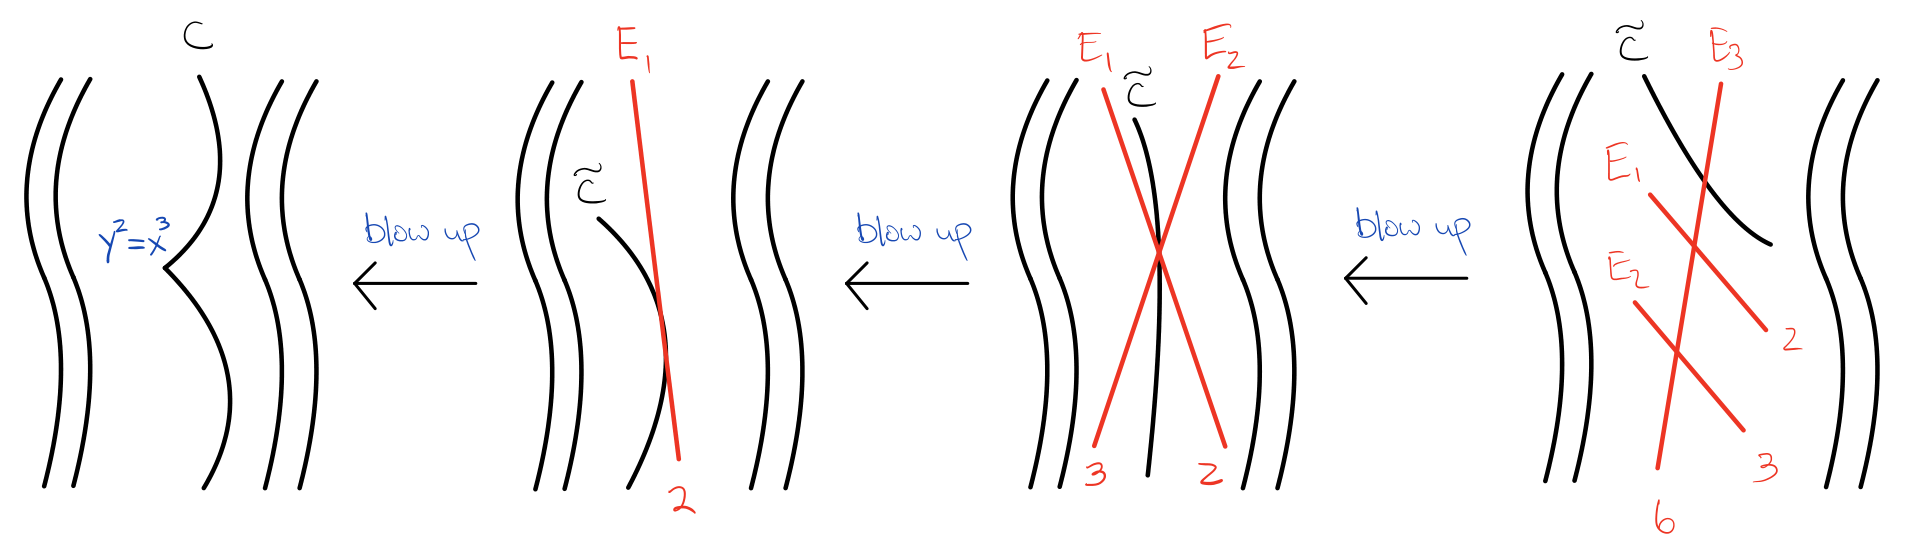
\includegraphics[width=.86\textwidth]{figures/reduction-step3.png}};
\begin{scope}[x={(im.south east)},y={(im.north west)}]
\fill[white] (0.185,0.52) rectangle (0.26,0.65);
\fill[white] (0.44,0.52) rectangle (0.52,0.65);
\fill[white] (0.7,0.52) rectangle (0.78,0.65);
\node[fill=white,inner sep=1pt,font=\scriptsize,text=blue] at (0.21,0.59) {爆破};
\node[fill=white,inner sep=1pt,font=\scriptsize,text=blue] at (0.477,0.59) {爆破};
\node[fill=white,inner sep=1pt,font=\scriptsize,text=blue] at (0.737,0.59) {爆破};
\end{scope}\end{tikzpicture}
